\documentclass[../../main.tex]{subfiles}
\begin{document}

{\bf [解]}
題意の式
\begin{align}
\begin{cases}
ab+1 \le abc \le bc+ca+ab+1 \\
a > b > c 
\end{cases} \label{eq:1}
\end{align}
を考える．

\cref{eq:1}の第一式の両辺を $abc$ でわって
\begin{align}
\dfrac{1}{c} + \dfrac{1}{abc} \le 1 \le \dfrac{1}{a} + \dfrac{1}{b} + \dfrac{1}{c} + \dfrac{1}{abc} \quad \cdots \text{③} \label{eq:2}
\end{align}
である．
簡単のため$T = \dfrac{1}{abc}$ とおく．
$c=1$ は\cref{eq:2}の左側の不等号が成立せず不適だから $c \ge 2$ が必要である．
\cref{eq:2}の右側の不等号に\cref{eq:1}の第二式を用いると
\begin{align}
1 \le \dfrac{1}{a} + \dfrac{1}{b} + \dfrac{1}{c} + \dfrac{1}{abc} < \dfrac{3}{c} + \dfrac{1}{c^3} \\
 \therefore 
c^3 - 3c^2 - 1 < 0 \quad (\because c > 0) \quad \cdots \text{④} \label{eq:3}
\end{align}
となる．まずはこれを満たす$c$を探す．
そのため$f(x) = x^3 - 3x^2 - 1$ とおく．$f'(x) = 3x^2 - 6x = 3x(x-2)$ より増減表は以下のようになる．

\begin{table}[htb]
\centering
\caption{$f(x)$ の増減表}
\label{tab:variation}
\begin{tabular}{c|cccccccccc}
$x$ & $-\infty$ & $\cdots$ & $0$ & $\cdots$ & $2$ & $\cdots$ & $3$ & $\cdots$ & $4$ & $\cdots$ \\ \hline
$f'(x)$ & & $+$ & $0$ & $-$ & $0$ & $+$ & $+$ & $+$ & $+$ & \\ \hline
$f(x)$  & & $\nearrow$ & $-1$ & $\searrow$ & $-5$ & $\nearrow$ & $-1$ & $\nearrow$ & $15$ & 
\end{tabular}
\end{table}

\begin{figure}[htb]
 \begin{center}
  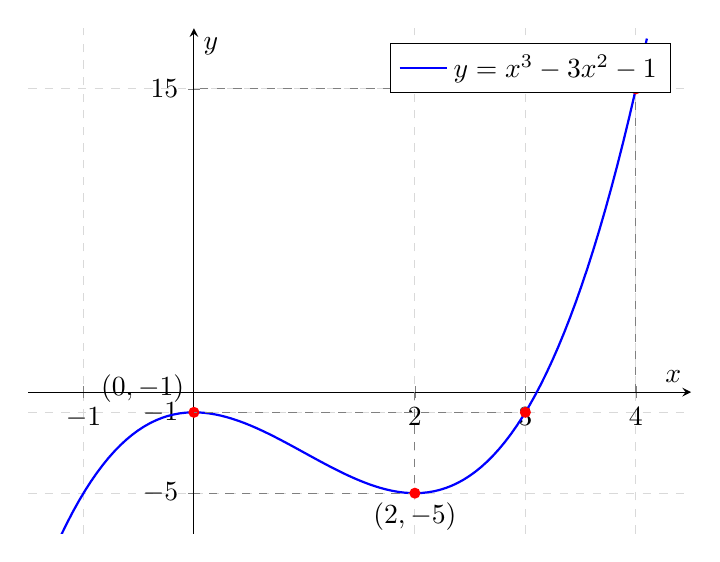
\begin{tikzpicture}
\begin{axis}[
    width=10cm,
    height=8cm,
    axis lines = center,
    xlabel = {$x$},
    ylabel = {$y$},
    xmin = -1.5, xmax = 4.5,
    ymin = -7, ymax = 18,
    xtick = {-1, 0, 2, 3, 4},
    ytick = {-5, -1, 0, 15},
    legend pos = north east,
    domain = -1.2:4.1,
    samples = 100,
    grid = major,
    grid style = {dashed, gray!30}
]

% y = x^3 - 3x^2 - 1
\addplot [thick, blue] {x^3 - 3*x^2 - 1};
\addlegendentry{$y = x^3 - 3x^2 - 1$};

% 極大値・極小値・特徴的な点の補助線とプロット
% 極大値 (0, -1)
\fill [red] (axis cs:0,-1) circle (2pt) node[above left, black] {$(0, -1)$};

% 極小値 (2, -5)
\draw [dashed, gray] (axis cs:2,0) -- (axis cs:2,-5) -- (axis cs:0,-5);
\fill [red] (axis cs:2,-5) circle (2pt) node[below, black] {$(2, -5)$};

% x = 3 での値 (3, -1)
\draw [dashed, gray] (axis cs:3,0) -- (axis cs:3,-1) -- (axis cs:0,-1);
\fill [red] (axis cs:3,-1) circle (2pt);

% x = 4 での値 (4, 15)
\draw [dashed, gray] (axis cs:4,0) -- (axis cs:4,15) -- (axis cs:0,15);
\fill [red] (axis cs:4,15) circle (2pt);

\end{axis}
\end{tikzpicture}
\caption{$y=f(x)$の概形．}
 \end{center}
\end{figure}

したがって $f(c)<0$ かつ$c \ge 2$を満たす$c$は$c=2,3$のみである．

\subparagraph{$1^\circ \ c=2$の時}
\cref{eq:1}に$c=2$を代入すると
\begin{align}
\begin{cases}
\dfrac{1}{2ab} \le \dfrac{1}{2} \le \dfrac{1}{a} + \dfrac{1}{b} + \dfrac{1}{2ab} \\
3 \le b < a
\end{cases} \label{eq:4}
\end{align}
である．\cref{eq:4}の第一式の右側の不等号に$b<a$を用いると
\begin{align}
\dfrac{1}{2} < \dfrac{2}{b} + \dfrac{1}{2b^2} \quad \therefore b^2 - 4b - 1 < 0
\end{align}
である．下図からわかるように，これと$3 \le b$を満たす$b$は $b=3, 4$ である．

\begin{figure}[htb]
\begin{center}
\begin{tikzpicture}
\begin{axis}[
    width=10cm, height=7cm,
    axis lines = center,
    xlabel = {$x$}, ylabel = {$y$},
    xmin = -1, xmax = 6,
    ymin = -6, ymax = 6,
    xtick = {0, 1, 2, 3, 4, 5},
    ytick = {-5, -4, -1, 0, 4},
    % y=0 (x軸) との交点を追加
    extra x ticks={4.236}, 
    extra x tick labels={$2+\sqrt{5}$},
    extra x tick style={tick label style={below right, font=\footnotesize}},
    grid = major,
    grid style = {dashed, gray!30},
    domain = -0.5:5.5,
    samples = 100,
    legend pos = north east,
]

% 不等式 f(x) < 0 の領域を塗りつぶし
\addplot[name path=f, thick, blue] {x^2 - 4*x - 1};
\addplot[name path=axis, draw=none, domain=-1:6] {0};
\addplot[blue, opacity=0.1] fill between[of=f and axis, soft clip={domain=-0.236:4.236}];

% 特徴的な点のプロットと補助線
% 頂点 (2, -5)
\draw [dashed, gray] (axis cs:2,0) -- (axis cs:2,-5) -- (axis cs:0,-5);
\fill [red] (axis cs:2,-5) circle (2pt);

% b=3 のとき (3, -4)
\draw [dashed, gray] (axis cs:3,0) -- (axis cs:3,-4) -- (axis cs:0,-4);
\fill [red] (axis cs:3,-4) circle (2pt);

% b=4 のとき (4, -1)
\draw [dashed, gray] (axis cs:4,0) -- (axis cs:4,-1) -- (axis cs:0,-1);
\fill [red] (axis cs:4,-1) circle (2pt);

% b=5 のとき (5, 4)
\draw [dashed, gray] (axis cs:5,0) -- (axis cs:5,4) -- (axis cs:0,4);
\fill [red] (axis cs:5,4) circle (2pt);

\addlegendentry{$y = x^2-4x-1$}
\end{axis}
\end{tikzpicture}
\end{center}
\caption{$y=x^2-4x-1$ のグラフ．$3 \le x < 2+\sqrt{5}$ の範囲にある整数は $x=3, 4$ のみである．}
\end{figure}

そこでさらに以下この2パターンについて考える．

\subparagraph{(I) $b=4$の時}
\cref{eq:4}に$b=4$を代入して
\begin{align}
 \dfrac{1}{8a} \le \dfrac{1}{2} \le \dfrac{1}{4} + \dfrac{1}{a} + \dfrac{1}{8a} = \dfrac{1}{4} + \dfrac{9}{8a} \\
\therefore 
 \dfrac{1}{4} \le a \le \dfrac{9}{2}
\end{align}
だが $5 \le a$ と矛盾するため不適である．

\subparagraph{(II) $b=3$の時}
\cref{eq:4}に$b=3$を代入して
\begin{align}
 \dfrac{1}{6a} \le \dfrac{1}{2} \le \dfrac{1}{3} + \dfrac{1}{a} + \dfrac{1}{6a} = \dfrac{1}{3} + \dfrac{7}{6a} \\
\therefore 
 \dfrac{1}{3} \le a \le 7
\end{align}
$4 \le a$ とあわせて$a=4, 5, 6, 7$が必要である．
逆にこの時，\cref{eq:1}は満たされる．

\subparagraph{$2^\circ \ c=3$}
\cref{eq:1}に$c=3$を代入すると
\begin{align}
\begin{cases}
\dfrac{1}{3ab} \le \dfrac{2}{3} \le \dfrac{1}{a} + \dfrac{1}{b} + \dfrac{1}{3ab} & \cdots \text{⑥} \\
4 \le b < a
\end{cases} \label{eq:5}
\end{align}
を得る．
\cref{eq:5}の第一式の右側の不等号に$b<a$を用いると
\begin{align}
\dfrac{2}{3} < \dfrac{2}{b} + \dfrac{1}{3b^2} \quad \therefore 2b^2 - 6b - 1 < 0
\end{align}
であり，下図からこれと$4<b$を満たす $b$ はないため不適である．

\begin{figure}[htb]
\begin{center}
\begin{tikzpicture}
\begin{axis}[
    width=10cm, height=7cm,
    axis lines = center,
    xlabel = {$x$}, ylabel = {$y$},
    xmin = -1, xmax = 5,
    ymin = -6, ymax = 10,
    xtick = {0, 1, 2, 3, 4},
    ytick = {-5.5, -1, 0, 7},
    % y=0 (x軸) との交点を追加
    extra x ticks={3.158}, 
    extra x tick labels={$\dfrac{3+\sqrt{11}}{2}$},
    extra x tick style={tick label style={below right, font=\footnotesize}},
    grid = major,
    grid style = {dashed, gray!30},
    domain = -0.7:4.3,
    samples = 100,
    legend pos = north east,
]

% 不等式 f(x) < 0 の領域を塗りつぶし
\addplot[name path=f, thick, green!60!black] {2*x^2 - 6*x - 1};
\addplot[name path=axis, draw=none, domain=-1:5] {0};
\addplot[green!60!black, opacity=0.1] fill between[of=f and axis, soft clip={domain=-0.158:3.158}];

% 特徴的な点のプロットと補助線
% 頂点 (1.5, -5.5)
\draw [dashed, gray] (axis cs:1.5,0) -- (axis cs:1.5,-5.5) -- (axis cs:0,-5.5);
\fill [red] (axis cs:1.5,-5.5) circle (2pt);

% x=3 のとき (3, -1)
\draw [dashed, gray] (axis cs:3,0) -- (axis cs:3,-1) -- (axis cs:0,-1);
\fill [red] (axis cs:3,-1) circle (2pt);

% b=4 のとき (4, 7) -> 領域外であることを明示
\draw [dashed, gray] (axis cs:4,0) -- (axis cs:4,7) -- (axis cs:0,7);
\fill [red] (axis cs:4,7) circle (2pt);

\addlegendentry{$y = 2x^2-6x-1$}
\end{axis}
\end{tikzpicture}
\end{center}
\caption{$y=2x^2-6x-1$ のグラフ．$x > \dfrac{3+\sqrt{11}}{2} (\approx 3.16)$ では常に $y>0$ であり，$x \ge 4$ に解はない．}
\end{figure}

以上で全ての場合分けが尽くされた．よって求める答えは
\begin{align}
(a,b,c) = (4,3,2), (5,3,2), (6,3,2), (7,3,2)
\end{align}
である．


\end{document}
